\documentclass[12pt]{amsart}

\usepackage{amsmath}
\usepackage{enumerate}
\usepackage[margin=1in]{geometry}
\usepackage{graphicx}
\graphicspath{{../imgs/}}

\openup 5pt

\author[Blake Farman]{Blake Farman\\University of South Carolina}
\title[Exam 03]{Math 111\\Exam 03}
\date{November 30, 2017}

\pdfpagewidth 8.5in
\pdfpageheight 11in
\usepackage[margin=1in]{geometry}

\theoremstyle{definition}
\newtheorem{thm}{}
\renewcommand{\qedsymbol}{}

\begin{document}
\maketitle

\begin{center}
  \fbox{\fbox{\parbox{5.5in}{\centering
        Answer the questions in the spaces provided on the
        question sheets and turn them in at the end of the class period.
        If you require extra space, use the back of the page and indicate that you have done so.
        
        Unless otherwise stated, all supporting work is required.
        Unsupported or otherwise mysterious answers will \textbf{not receive credit.}
        
        You may use a calculator, but you may \textbf{not} use a Computer Algebra System (CAS)
        or any other electronic device whatsoever, \textbf{including cell phones.}
        By writing your name on the line below, you indicate that you have read and understand these directions.}}}
\end{center}

\vspace{0.2in}
\makebox[\textwidth]{Name: Solutions}
\vspace{0.2in}

$$
\begin{array}{|c|c|c|}
  \hline
  \text{Problem} & \text{Points Earned} & \text{Points Possible}\\
  \hline
  1 & & 3\\
  \hline
  2 & & 4\\
  \hline
  3 & & 3\\
  \hline
  4 & & 5\\
  \hline
  5 & & 10 \\
  \hline
  6 & & 20\\
  \hline
  7 & & 10\\
  \hline
  8 & & 10\\
  \hline
  9 & & 10\\
  \hline
  10 & & 10\\
  \hline
  11 & & 15\\
  \hline
  \text{Total} & & 100\\
  \hline
\end{array}
$$

\newpage

\section{Definitions}

\begin{thm}[3 Points]
  Let $a$ be a fixed positive number.
  The base $a$ logarithm of $x$ is defined by
  \vspace{.25in}
  $$\log_a(x) = y\  \text{if and only if}\ x = a^y.$$
\end{thm}

\begin{thm}[4 Points]
  Let $a$ be a positive number.  Fill in the blanks.
  \begin{enumerate}[(a)]
  \item
    \vspace{.25in}
    $\displaystyle{\log_a(1) = 0}$.
    \vspace{.25in}
  \item
    $\displaystyle{\log_a(a) = 1}$.
    \vspace{.25in}
  \item
    $\displaystyle{\log_a(a^x) = x}$.
    \vspace{.25in}
  \item
    $\displaystyle{a^{\log_a(x)} = x}$.
  \end{enumerate}
  \vspace{.5in}
\end{thm}

\begin{thm}[3 Points]
  Let $0 < a$ and $C$ be fixed numbers.  Fill in the blanks.
  \begin{enumerate}[(a)]
  \item
    \vspace{.25in}
    $\displaystyle{\log_a(xy) = \log_a(x) = \log_a(y)}$.
    \vspace{.25in}
  \item
    $\displaystyle{\log_a\left(\frac{x}{y}\right) = \log_a(x) - \log_a(y)}$.
    \vspace{.25in}
  \item
    $\displaystyle{\log_a(x^C) = C\log_a(x)}$.
  \end{enumerate}
  \vspace{.25in}
\end{thm}

\begin{thm}[5 Points]
  Let $a$ and $b$ be fixed positive numbers.
  Use the Change of Base formula to rewrite $\log_a(x)$ with base $b$.
  \vspace{.12in}
  $$\log_a(x) = \frac{\log_b(x)}{\log_b(a)}$$
  \vspace{.12in}
\end{thm}

\newpage

\section{Problems}

\begin{thm}[10 Points]
  Compute the following logarithms.
  \begin{enumerate}[(a)]
  \item
    $\log_{4}(64)$.
    \begin{proof}[Solution]
      \begin{eqnarray*}
        \log_4(64) &=& \log_4(2^6)\\
        &=& \log_4(2^{2\cdot 3})\\
        &=& \log_4((2^2)^3)\\
        &=& \log_4(4^3)\\
        &=& 3.
      \end{eqnarray*}
    \end{proof}
  \item
    $\log_{5}(125)$.
    \begin{proof}[Solution]
      \begin{eqnarray*}
        \log_5(125) &=& \log_5(5^3)\\
        &=& 3.
      \end{eqnarray*}
    \end{proof}
  \item
    $\log_{81}(9)$.
    \begin{proof}[Solution]
      \begin{eqnarray*}
        \log_{81}(9) &=& \log_{81}(\sqrt{81})\\
        &=& \log_{81}(81^{\frac{1}{2}})\\
        &=& \frac{1}{2}\log_{81}(81)\\
        &=& \frac{1}{2}.
      \end{eqnarray*}
    \end{proof}
  \item
    $\log_{16}(32)$.
    \begin{proof}[Solution]
      \begin{eqnarray*}
        \log_{16}(32) &=& \frac{\log_2(32)}{\log_2(16)}\\
        &=& \frac{\log_2(2^5)}{\log_2(2^4)}\\
        &=& \frac{5}{4}.
      \end{eqnarray*}
    \end{proof}
  \end{enumerate}
\end{thm}

\begin{thm}[20 Points]
  \begin{enumerate}[(a)]
  \item
    Simplify the expression 
    $$\log_6(x - 5) - 2\log_6\left(\frac{1}{\sqrt{x}}\right)$$
    \begin{proof}[Solution]
      \begin{eqnarray*}
        \log_6(x - 5) - 2\log_6\left(\frac{1}{\sqrt{x}}\right) &=& \log_6(x - 5) - 2\log_6(x^{-\frac{1}{2}})\\
        &=& \log_6(x - 5) - 2\left(-\frac{1}{2}\right)\log_6(x)\\
        &=& \log_6(x - 5) + \log_6(x)\\
        &=& \log_6((x - 5)x)\\
        &=& \log_6(x^2 - 5x)
      \end{eqnarray*}
    \end{proof}
  \item
    Solve the following equation for $x$.
    $$\log_6(x - 5) - 2\log_6\left(\frac{1}{\sqrt{x}}\right) = 1$$
    
    \begin{proof}[Solution]
      From part (a) we have
      $$\log_6(x^2 - 5x) = 1$$
      so applying the function $6^x$ to both sides we have
      $$6 = 6^{\log_6(x^2 - 5x)} = x^2 - 5x.$$
      Subtracting 6 from both sides we are left to solve the equation
      $$x^2 - 5x - 6 = 0.$$
      Factoring the left hand side we have
      $$x^2 - 5x - 6 = (x - 6)(x + 1) = 0$$
      and thus either $x = 6$ or $x = -1$.
      We notice that $-1$ is not in the domain of $\log_6(x - 5)$, since the logarithm is only defined for positive numbers, hence $x = -1$ is an extraneous solution.
      Therefore the only solution is $x = 6$.
    \end{proof}
  \end{enumerate}
\end{thm}

\begin{thm}[10 Points]
  Solve the following equation for $x$.
  $$2^{x^2} = \frac{4}{2^x}$$
\end{thm}

\begin{proof}[Solution]
  Multiplying both sides by $2^x$ we obtain
  $$2^{x^2}2^x = 2^{x^2 + x} = 4.$$
  Applying $\log_2(x)$ to both sides yields the equation
  $$x^2 + x = \log_2(2^{x^2 + x}) = \log_2(4) = 2.$$
  Subtracting 2 from both sides we are left to solve
  $$x^2 + x - 2 = 0.$$
  Factoring the left hand side we see
  $$x^2 + x - 2 = (x - 1)(x + 2) = 0$$
  implies that either $x = 1$ or $x = -2$.
\end{proof}

\begin{thm}[10 Points]
  Let $f(x) = x^2 - 6x - 40$.
  \begin{enumerate}[(a)]
  \item
    By completing the square, write $f(x)$ in vertex form.
    \begin{proof}[Solution]
      \begin{eqnarray*}
        f(x) &=& x^2 - 6x - 40\\
        &=& (x^2 - 2(3)x + 3^2) - 3^2 - 40\\
        &=& (x - 3)^2 - 9 - 40\\
        &=& (x - 3)^2 - 49.
      \end{eqnarray*}
    \end{proof}
  \item
    Find the solutions to $f(x) = 0$.
    \begin{proof}[Solution]
      We can factor
      $$0 = x^2 - 6x - 40 = (x - 10)(x + 4)$$
      so the solutions are $x = 10$ and $x = -4$.
    \end{proof}
  \item
    Find the coordinates of the $y$-intercept for $f(x)$.
    \begin{proof}[Solution]
      The $y$-intercept is the point
      $$(0,f(0)) = (0, 0^2 - 6(0) - 40) = (0, -40).$$
    \end{proof}
  \end{enumerate}
\end{thm}

\begin{thm}[10 Points]
  Sketch a graph of $f(x) = x^2 - 6x - 40.$
  Label the $y$-intercept, the vertex, and any $x$-intercepts.
\end{thm}
\begin{proof}[Solution]\hfill\\
  
  \begin{center}
    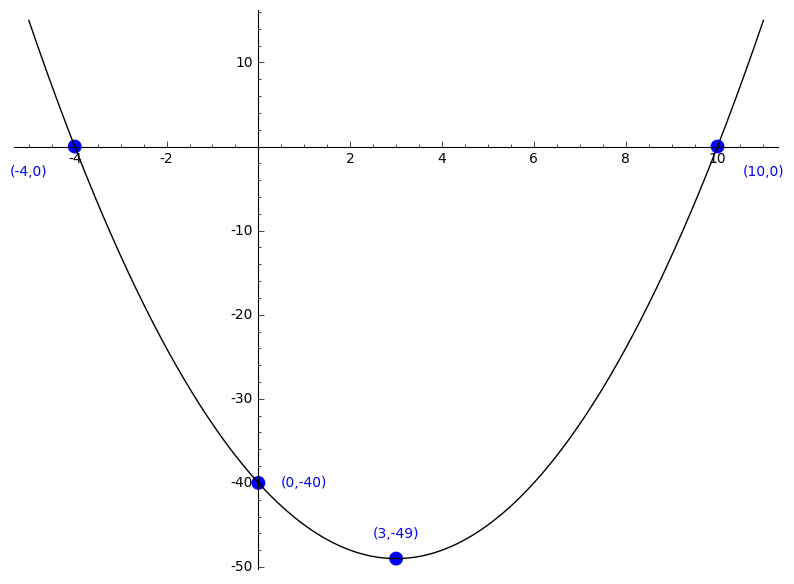
\includegraphics[scale=0.8]{parabola}
  \end{center}
\end{proof}

\noindent Alice tosses a ball straight up in the air.
When she releases the ball, it leaves her hand at a velocity of 32 feet/sec.
The height of the ball relative to Alice's hand after $t$ seconds can be modeled by the function
$$h(t) = -16t^2 + 32t.$$
Use this model to answer the following questions.

\begin{thm}[10 Points]
Sketch a graph of this function, labeling the vertical intercept, the horizontal intercepts, and the vertex.
What do the horizontal intercepts and the vertex represent?
\end{thm}

\begin{proof}[Solution]\hfill\\
  \begin{center}
    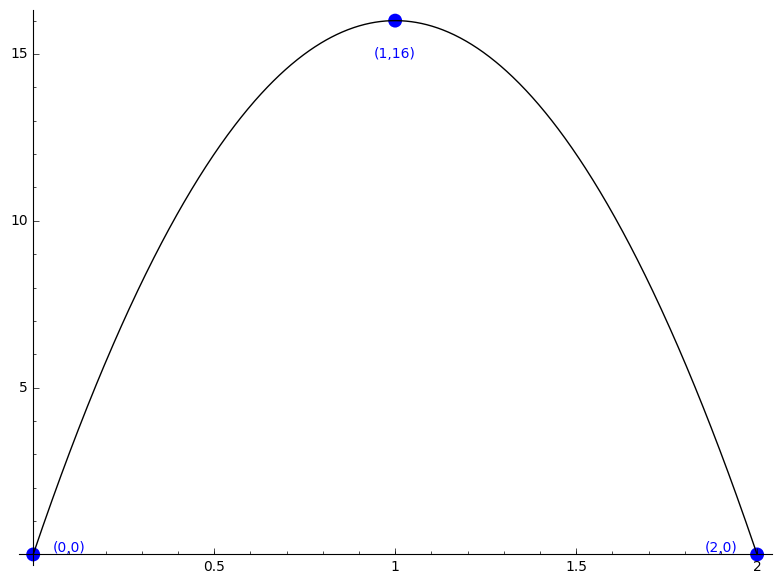
\includegraphics[scale = .8]{kinematics}
  \end{center}

  The left-most horizontal intercept represents the initial position of the ball (in Alice's hand).
  The right-most horizontal intercept represents the time when the ball returns to Alice's hand.
  The vertex represents the maximum height of the ball.
\end{proof}

\begin{thm}[15 Points]
    \begin{enumerate}[(a)]
  \item
    After how many seconds does the ball reach its maximum height?
    \begin{proof}[Solution]
      The ball reaches its maximum height after 1 second has elapsed; this is the $t$-coordinate of the vertex.
    \end{proof}
  \item
    What is the maximum height attained by the ball?
    \begin{proof}[Solution]
      The maximum height reached by the ball is 16 feet; this is the $h$-coordinate of the vertex.
    \end{proof}
  \item
    After how many seconds does the ball return to Alice's hand?
    \begin{proof}[Solution]
      The ball returns to Alices hand after 2 seconds; this is the $t$-coordinate of the second horizontal intercept.
    \end{proof}
  \end{enumerate}
\end{thm}
\end{document}
